\documentclass{article}
\usepackage{amsmath}
\usepackage{tikz-cd}

\begin{document}

Axiom 4) of Definition \ref{def:operad} for the endomorphism operad $\mathcal{O}\textup{End}(X)$: Applying $f$ to arguments of the form $\tau_{\sigma_i}(g_i)$ yields the same function as first permuting all arguments via $(\sigma_1,\ldots,\sigma_{n})^{-1}$ and then applying $f \star \vec{g}$.

\[
\begin{tikzcd}[column sep=small]
f \left[ \begin{array}{c}
\begin{tikzpicture}[baseline=(current bounding box.center)]
\node (a) at (0,0) {$f$};
\draw[->] (a) -- ++(0,0.5);
\end{tikzpicture} \\
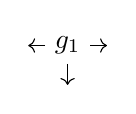
\begin{tikzpicture}[baseline=(current bounding box.center)]
\node (a) at (0,0) {$g_1$};
\draw[->] (a) -- ++(0,-0.5);
\draw[->] (a) -- ++(-0.5,0);
\draw[->] (a) -- ++(0.5,0);
\end{tikzpicture} \quad \cdots \quad 
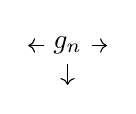
\begin{tikzpicture}[baseline=(current bounding box.center)]
\node (a) at (0,0) {$g_n$};
\draw[->] (a) -- ++(0,-0.5);
\draw[->] (a) -- ++(-0.5,0);
\draw[->] (a) -- ++(0.5,0);
\end{tikzpicture}
\end{array} \right] f \star \vec{g} \\
\tau_{\sigma_1}(g_1) \left[ \begin{array}{c}
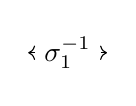
\begin{tikzpicture}[baseline=(current bounding box.center)]
\node (a) at (0,0) {$\sigma_1^{-1}$};
\draw[->] (a) -- ++(-0.5,0);
\draw[->] (a) -- ++(0.5,0);
\end{tikzpicture} \quad \sigma_n^{-1} \quad 
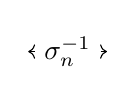
\begin{tikzpicture}[baseline=(current bounding box.center)]
\node (a) at (0,0) {$\sigma_n^{-1}$};
\draw[->] (a) -- ++(-0.5,0);
\draw[->] (a) -- ++(0.5,0);
\end{tikzpicture}
\end{array} \right] (\sigma_1,\ldots,\sigma_n)^{-1}
\end{tikzcd}
\]

\end{document}